\documentclass{mitaoeminorreportty}

\usepackage{amsmath,amssymb,amsfonts}
\usepackage{graphicx}
\usepackage{booktabs}
\usepackage{multirow}
\usepackage{listings}
\usepackage{xcolor}
\usepackage{hyperref}
\usepackage{geometry}
\usepackage{tikz}
\usetikzlibrary{shapes.geometric, arrows, positioning}

\hypersetup{
    colorlinks=true,
    linkcolor=black,
    citecolor=blue,
    urlcolor=blue
}

% Code Listing Configuration
\definecolor{codegreen}{rgb}{0,0.6,0}
\definecolor{codegray}{rgb}{0.5,0.5,0.5}
\definecolor{codepurple}{rgb}{0.58,0,0.82}
\definecolor{backcolour}{rgb}{0.97,0.97,0.98}

\lstdefinestyle{mystyle}{
    backgroundcolor=\color{backcolour},   
    commentstyle=\color{codegreen},
    keywordstyle=\color{blue},
    numberstyle=\tiny\color{codegray},
    stringstyle=\color{codepurple},
    basicstyle=\ttfamily\footnotesize,
    breakatwhitespace=false,         
    breaklines=true,                 
    captionpos=b,                    
    keepspaces=true,                 
    numbers=left,                    
    numbersep=5pt,                  
    showspaces=false,                
    showstringspaces=false,
    showtabs=false,                  
    tabsize=2
}
\lstset{style=mystyle}

\begin{document}

\projecttitle{SecureBank: An Architectural Framework for Enterprise Digital Banking with Dual-Engine Persistence and Administrative Governance}

\student{Atharva Kamble}{202401100057}
\student{Aaditi Bhalerao}{202401100058}
\student{Group Member 3}{PRN3}
\student{Group Member 4}{PRN4}

\department{Software Engineering}
\projectadvisor{Name of Project Guide} %%% Write the name of Guide Here
\projectcoordinator{Mrs. Gauri Thite}
\dean{Dr. Manish Giri}
\academicyear{2026--2027}

\pagestyle{empty}
\titlepage
\certificate
\declaration

\newpage
\pagestyle{plain}
\pagenumbering{roman}
\setcounter{page}{4}

\chapter*{Abstract}
\addcontentsline{toc}{chapter}{Abstract}

In the era of modern digital finance, web applications require stringent security standards, high-throughput asynchronous request handling, and fault-tolerant persistent storage without compromising user experience. This report presents \textbf{SecureBank}, an enterprise-grade digital banking simulation platform engineered with a decoupled full-stack architecture. 

The frontend utilizes a modern Single-Page Application (SPA) built with React 19 and bundled via Vite, integrating an architectural design system inspired by the Aceternity Studio specification featuring dashed blueprint gridlines, floating glassmorphic navigation, and responsive bento cards. The backend is implemented in Node.js and Express 5, implementing a multi-layered security pipeline including 12-round salted key derivation using Bcrypt, cryptographic session handling via signed \texttt{httpOnly} cookies, and role-based access control (RBAC).

A cornerstone innovation of SecureBank is its \textbf{Dual-Engine Persistence Layer}, which prioritizes a cloud-native MongoDB document store managed through the Mongoose Object-Document Mapper (ODM) with automatic failover to an embedded SQLite database configured with Write-Ahead Logging (WAL). This guarantees zero application crashes in disconnected or local developer environments while supporting high-throughput cloud environments such as MongoDB Atlas. Furthermore, a dedicated Administrative Control Plane provides real-time transaction ledger auditing, customer lifecycle governance, and manual liquidity adjustments. The platform is configured for serverless execution on Vercel via reverse proxy trust and centralized session persistence.

\vspace{0.8cm}
\noindent \textbf{Keywords:} Financial Technology, Single-Page Application, React 19, Express.js, Bcrypt, Session Security, MongoDB, Dual-Engine Persistence, Serverless Architecture, Role-Based Access Control.

\chapter*{Acknowledgement}
\addcontentsline{toc}{chapter}{Acknowledgement}

We take this opportunity to express our profound gratitude and deep regards to our Project Guide, for their exemplary guidance, monitoring, and constant encouragement throughout the development of the \textbf{SecureBank} project. The constructive feedback and technical directions provided were invaluable in surmounting the complex engineering challenges encountered during system design and implementation.

We express our sincere thanks to \textbf{Mrs. Gauri Thite}, Project Coordinator, for her consistent support, schedule planning, and coordination during the project tenure.

We also extend our earnest appreciation to \textbf{Dr. Manish Giri}, Dean, Department of Software Engineering, MIT Academy of Engineering (MITAOE), for providing the necessary infrastructural facilities, laboratory resources, and conducive academic environment that enabled the successful completion of this project.

Finally, we express our heartfelt thanks to our parents, fellow students, and faculty members who directly or indirectly aided us in bringing this endeavor to fruition.

\vspace{1.5cm}
\begin{flushright}
\textbf{Atharva Kamble} (PRN: 202401100057) \\
\textbf{Aaditi Bhalerao} (PRN: 202401100058) \\
\textbf{Group Member 3} (PRN: PRN3) \\
\textbf{Group Member 4} (PRN: PRN4) \\
\vspace{0.3cm}
Department of Software Engineering \\
MIT Academy of Engineering, Pune
\end{flushright}


\setcounter{tocdepth}{3}
\tableofcontents

\newpage
\listoffigures

\newpage
\listoftables

\newpage
\pagenumbering{arabic}

\chapter{Introduction}

\section{Background and Overview}
The global financial landscape has experienced an unprecedented transition from physical, branch-centric operations to ubiquitous digital banking platforms. Modern users demand instant, frictionless financial interactions accessible across various computing devices. However, this convenience introduces substantial engineering hurdles: ensuring ironclad security for sensitive customer assets, preventing unauthorized transaction replay, maintaining continuous availability, and delivering intuitive, responsive user interfaces.

Traditional financial platforms often struggle with legacy monolithic designs, brittle relational database dependencies, and cluttered user interfaces that introduce user fatigue. \textbf{SecureBank} addresses these challenges by reimagining digital banking through a decoupled client-server architecture built on modern JavaScript/TypeScript paradigms. The system combines an ultra-modern aesthetic inspired by the Aceternity Studio design philosophy with a hardened Node.js/Express application core backed by a resilient dual-engine persistence layer.

\section{Motivation}
The impetus behind developing SecureBank stems from three primary observations in contemporary financial software engineering:
\begin{enumerate}
    \item \textbf{Vulnerability of Standard Web Systems:} Many simulation or academic banking frameworks store passwords in plaintext or employ obsolete hashing algorithms (such as MD5 or SHA-1) vulnerable to rainbow table attacks and collision exploitation. There is a pressing need for reference implementations utilizing salted adaptive key derivation (Bcrypt) and secure HTTP cookie architectures.
    \item \textbf{Brittle Database Coupling:} Many applications crash upon initialization if their primary cloud or distributed database cluster experiences network partitions or offline developer scenarios. An engineering pattern that provides transparent fallback to a fast embedded engine (SQLite) preserves developer productivity while ensuring cloud scalability (MongoDB).
    \item \textbf{Cognitive Friction in Financial Interfaces:} Traditional banking interfaces suffer from visual bloat and disorganized information architecture. Designing a high-trust interface using architectural framing, clear typography, and responsive state management establishes immediate user confidence.
\end{enumerate}

\section{Problem Statement}
To design, implement, and deploy an enterprise-ready digital banking simulation system that provides:
\begin{itemize}
    \item Robust customer onboarding with strict cryptographic password hashing and schema validation.
    \item Synchronous double-entry transaction processing with atomic balance enforcement to eliminate drift.
    \item An administrative governance portal for real-time liquidity management, customer monitoring, and global audit logging.
    \item A resilient data persistence pipeline supporting MongoDB as the primary document store with automatic, crash-free fallback to an embedded SQLite database.
    \item A cloud-ready deployment configuration suitable for modern serverless container execution (Vercel).
\end{itemize}

\section{Project Objectives}
The core objectives of the SecureBank project are as follows:
\begin{enumerate}
    \item \textbf{Cryptographic Security:} Implement 12-round salted Bcrypt password encryption, secure session regeneration on privilege elevation, and \texttt{httpOnly} cookie transmission to mitigate XSS and CSRF threats.
    \item \textbf{Dual-Engine Storage Abstraction:} Construct a unified Data Access Layer (\texttt{dbService}) that automatically routes operations to MongoDB (via Mongoose) when connected, or falls back to an embedded SQLite database without throwing unhandled connection exceptions.
    \item \textbf{Atomic Transaction Enforcement:} Guarantee that balance recalculations and transaction ledger entries occur as atomic units, ensuring zero ledger drift during simulated debits or credits.
    \item \textbf{Administrative Control Center:} Provide an authorized administrative tier capable of querying system metrics, viewing all registered accounts, adjusting liquidity, and purging user accounts with cascading ledger cleanup.
    \item \textbf{Modern High-Trust Frontend:} Implement a responsive React 19 SPA incorporating floating pill navigation, bento-grid layouts, dynamic virtual DOM updates, and custom CSS styling without external bloated UI component kits.
    \item \textbf{Continuous Deployment:} Configure the platform for automated cloud hosting via Vercel serverless lambda wrappers and GitHub synchronization.
\end{enumerate}

\section{Scope of the Project}
The scope of this project encompasses:
\begin{itemize}
    \item \textbf{User Module:} Customer self-registration, validation of 10-digit Indian mobile formats, ISO birthdates, unique email verification, secure session-based authentication, and account profile deletion.
    \item \textbf{Transaction Module:} Simulated debit and credit operations with instantaneous validation against available balances, generating immutable chronological activity records.
    \item \textbf{Administration Module:} Dedicated admin portal protected by role-based guards, supporting customer search, balance intervention, audit inspection, and account termination.
    \item \textbf{Database Module:} Mongoose schema definitions for MongoDB and table structures for SQLite with automatic data migration from local storage to cloud MongoDB upon initial synchronization.
\end{itemize}
\textit{Note on Exclusions:} SecureBank is an engineering prototype and simulation environment. It does not interface with actual Central Bank payment gateways (e.g., UPI, NEFT, RTGS) or real monetary assets.

\section{Organization of the Report}
The subsequent chapters of this report are structured as follows:
\begin{itemize}
    \item \textbf{Chapter 2 (Literature Survey):} Examines related work, existing open-source and commercial banking architectures, and highlights identified research and technical gaps.
    \item \textbf{Chapter 3 (System Requirements and Analysis):} Outlines functional and non-functional requirements, user personas, software/hardware prerequisites, and feasibility dimensions.
    \item \textbf{Chapter 4 (System Design and Architecture):} Details the overall multi-tier architectural framework, Data Flow Diagrams (DFDs), UML diagrams, and entity-relationship models.
    \item \textbf{Chapter 5 (Implementation Details):} Discusses the core algorithmic implementation, cryptographic routines, dual-engine data service logic, API endpoints, and frontend components.
    \item \textbf{Chapter 6 (Results, Testing, and Discussion):} Presents verification results, testing methodologies (functional, validation, security), comparative analysis, and concludes with future enhancements.
    \item \textbf{Appendix \& Bibliography:} Provides the API route specification, configuration instructions, and academic references.
\end{itemize}

\chapter{Literature Survey}

\section{Overview of Modern Financial Web Architecture}
Financial technology (FinTech) systems demand rigorous computational engineering. Over the past decade, architectural patterns have migrated from server-rendered multi-page applications (MPAs) toward decoupled Single-Page Applications (SPAs) communicating with RESTful or GraphQL microservices over Transport Layer Security (TLS). 

Research by Fielding \cite{fielding2000architectural} established the foundations of representational state transfer (REST), emphasizing stateless client-server interactions. In financial applications, maintaining state securely while preserving stateless communication requires robust session management mechanisms. Modern literature \cite{owasp2021top} highlights that token-based architectures (such as JSON Web Tokens stored in HTML5 LocalStorage) introduce severe vulnerabilities to Cross-Site Scripting (XSS) exploitation. Consequently, cryptographic cookie-based session stores managed via signed, \texttt{httpOnly}, and \texttt{SameSite} attributes remain the recommended gold standard for high-security banking gateways.

\section{Review of Existing Systems}
To establish the necessity and innovation of SecureBank, we reviewed three dominant paradigms in banking software engineering:

\subsection{Traditional Relational Monolithic Banking Portals}
Historically, digital banking was built on monolithic enterprise stacks (e.g., Java Enterprise Edition or ASP.NET) tightly coupled to centralized relational databases (e.g., Oracle Database or IBM DB2). While offering ACID (Atomicity, Consistency, Isolation, Durability) guarantees, these systems exhibit:
\begin{itemize}
    \item High deployment inertia and tight coupling between presentation and business logic.
    \item Severe performance degradation during horizontal scaling due to centralized locking contention.
    \item Cluttered and rigid user interfaces that lack mobile responsiveness.
\end{itemize}

\subsection{Standard Educational and Open-Source Banking Simulators}
Various academic and open-source banking simulators exist for didactic purposes (e.g., OWASP Juice Shop, WebGoat banking modules, and basic MERN repositories). An analysis of these systems reveals significant shortcomings:
\begin{itemize}
    \item Passwords are often encrypted with unkeyed MD5 or SHA-256 hashes without adaptive work factors, leaving them vulnerable to GPU-accelerated dictionary attacks.
    \item Database dependency is rigid: if a remote database URI is unreachable, the Node.js process immediately terminates with an uncaught exception (\texttt{ECONNREFUSED}).
    \item Lack of a centralized administrative oversight console to audit cross-customer transactions or dynamically adjust ledger anomalies.
\end{itemize}

\subsection{Cloud-Native Microservices Financial Architectures}
Enterprise platforms (such as Stripe, Revolut, and Monzo) utilize distributed event-driven microservices. While highly scalable, implementing such architectures for intermediate or agile projects introduces excessive operational overhead, network latency orchestration, distributed transaction failure modes (such as two-phase commit overhead), and substantial cloud infrastructure costs.

\section{Comparative Analysis of Related Systems}
Table \ref{tab:comparison} summarizes the comparative features of existing banking implementations against SecureBank.

\begin{table}[htbp]
\centering
\caption{Comparative Analysis of Banking Architecture Frameworks}
\label{tab:comparison}
\resizebox{\textwidth}{!}{%
\begin{tabular}{@{}lcccc@{}}
\toprule
\textbf{Feature / Metric} & \textbf{Legacy Monoliths} & \textbf{Open-Source Demos} & \textbf{Enterprise Microservices} & \textbf{SecureBank (Proposed)} \\ \midrule
Client Architecture & Server-Rendered MPA & Basic React/Vue SPA & Multi-Platform Micro-frontends & React 19 SPA (Vite Bundled) \\
UI Design Standard & Cluttered Tables & Generic Bootstrap/MUI & Proprietary Design System & Aceternity Architectural Studio \\
Password Security & Legacy Hash (SHA-1/256) & Plaintext / MD5 & Argon2 / Bcrypt & Bcrypt (12 Salt Rounds) \\
Session Management & In-Memory Server Sticky & LocalStorage JWT & Distributed Redis Clusters & Signed \texttt{httpOnly} + MongoStore \\
Database Coupling & Rigid SQL Engine & Hardcoded MongoDB & Distributed Polyglot & \textbf{Dual-Engine (Mongo + SQLite)} \\
Offline Tolerance & Nil (Crashes) & Nil (Unhandled Rejection) & Multi-Region Redundancy & \textbf{Automatic Zero-Crash Fallback} \\
Admin Control Plane & Separate Internal Tool & Usually Omitted & Complex Enterprise Dashboard & \textbf{Integrated RBAC Console} \\
Deployment Model & Bare Metal / VM & Localhost Only & Kubernetes / AWS ECS & \textbf{Serverless Cloud (Vercel)} \\ \bottomrule
\end{tabular}%
}
\end{table}

\section{Identified Technical Gaps}
From the literature and system analysis, three critical technical gaps were identified:
\begin{enumerate}
    \item \textbf{Absence of Dynamic Multi-Engine Failover in Intermediate Web Applications:} Almost all Node.js financial frameworks crash during startup if their target MongoDB daemon is unavailable. A lightweight, synchronous database adapter capable of falling back to embedded local storage with automatic data migration upon reconnection is virtually nonexistent in standard educational stacks.
    \item \textbf{Inadequate Administrative Intervention Tools:} Most banking prototypes focus entirely on the end-user customer flow while ignoring administrative governance, leaving no interface for ledger corrections, audit trail monitoring, or manual liquidity management.
    \item \textbf{Visual and Architectural Disconnect in Web Security:} Visual aesthetic is often treated as secondary to security. However, empirical user experience research shows that visual hierarchy, clear typographic cues, and minimal visual noise significantly reduce user operational error in financial workflows.
\end{enumerate}

\section{Summary}
The literature confirms that while advanced enterprise systems achieve high resilience at immense complexity and cost, entry-to-intermediate banking systems remain fragile and insecure. SecureBank bridges this divide by delivering enterprise security patterns (Bcrypt, \texttt{httpOnly} cookie sessions, dual-engine persistence) within an elegant, serverless-ready architectural framework.

\chapter{System Requirements and Analysis}

\section{Requirements Gathering and User Personas}
Requirements analysis was conducted by evaluating banking operational standards and defining two primary user personas:
\begin{enumerate}
    \item \textbf{Retail Banking Customer (Persona A):} An end-user seeking an intuitive web portal to register an account, inspect real-time available funds, simulate credit/debit transactions, and maintain account privacy.
    \item \textbf{System Administrator (Persona B):} A financial operations auditor requiring global visibility across all registered accounts, audit monitoring of system transactions, liquidity intervention capabilities, and administrative user management.
\end{enumerate}

\section{Functional Requirements}
The functional capabilities of SecureBank are categorized into four major subsystems:

\subsection{Customer Authentication and Account Management}
\begin{itemize}
    \item \textbf{FR-1 (Customer Onboarding):} The system shall provide a registration portal validating full name, unique email address, 10-digit mobile phone number, valid date of birth ($\le \text{current date}$), account type (Savings/Current), and a password of minimum 8 characters.
    \item \textbf{FR-2 (Initial Balance Provisioning):} Upon account creation, the system shall credit an initial demo balance of ₹10,000.
    \item \textbf{FR-3 (Secure Authentication):} The system shall authenticate customers via email and password using constant-time hash comparisons, issuing an encrypted session cookie.
    \item \textbf{FR-4 (Session Termination):} The system shall permit customers to log out, immediately destroying the server-side session and clearing client cookies.
    \item \textbf{FR-5 (Self-Service Deletion):} Customers shall be empowered to permanently purge their account and transaction ledger with cascading removal.
\end{itemize}

\subsection{Transaction and Ledger Management}
\begin{itemize}
    \item \textbf{FR-6 (Debit Simulation):} The system shall allow customers to initiate debit transactions, strictly enforcing that the requested amount does not exceed the customer's current balance.
    \item \textbf{FR-7 (Credit Simulation):} The system shall permit deposit transactions up to a safety threshold of ₹1,000,000 per transaction.
    \item \textbf{FR-8 (Atomic Balance Update):} Balance calculation and ledger insertion shall be executed atomically.
    \item \textbf{FR-9 (Transaction History Feed):} The customer dashboard shall render the 50 most recent transactions with type indicators (credit/debit), formatted currency, and localized timestamps.
\end{itemize}

\subsection{Administrative Control and Governance}
\begin{itemize}
    \item \textbf{FR-10 (Admin Authentication):} The system shall provide a dedicated admin entry point accepting administrative credentials (\texttt{admin} / \texttt{admin123}).
    \item \textbf{FR-11 (System Metric Aggregation):} The admin dashboard shall calculate and display total registered accounts, aggregate vault balance (sum of all balances), and total system transactions.
    \item \textbf{FR-12 (Customer Directory Search):} Admins shall be able to search and filter customer records dynamically by name, email, or telephone.
    \item \textbf{FR-13 (Administrative Balance Intervention):} Admins shall have the authority to credit or debit any customer account directly with an audit memorandum.
    \item \textbf{FR-14 (Administrative Account Revocation):} Admins shall be authorized to delete rogue or inactive customer accounts with cascading transaction removal.
    \item \textbf{FR-15 (Global Audit Stream):} The admin portal shall display an enterprise-wide ledger of transactions performed across all customer accounts.
\end{itemize}

\subsection{Dual-Engine Persistence}
\begin{itemize}
    \item \textbf{FR-16 (Primary MongoDB Persistence):} The system shall route all queries to MongoDB when reachable.
    \item \textbf{FR-17 (Secondary SQLite Failover):} If MongoDB is offline, the system shall automatically fallback to local embedded SQLite without terminating the application process.
    \item \textbf{FR-18 (Automatic Migration):} When an empty MongoDB instance connects, the system shall automatically migrate local SQLite records to MongoDB collections.
\end{itemize}

\section{Non-Functional Requirements}
\begin{itemize}
    \item \textbf{NFR-1 (Security):} Passwords shall never be stored in plaintext. They must be salted and hashed with a Bcrypt cost factor of 12. Sessions must use \texttt{httpOnly} and \texttt{SameSite} flags.
    \item \textbf{NFR-2 (Performance and Latency):} Client-side page navigation within the SPA shall be instantaneous ($<50$ ms). API response latency under local conditions shall remain below 100 ms.
    \item \textbf{NFR-3 (Reliability and Fault Tolerance):} In the event of primary database failure, the system must maintain 100\% uptime by shifting read/write operations to the secondary engine.
    \item \textbf{NFR-4 (Usability and Aesthetics):} The user interface must comply with the Aceternity Studio design standard, presenting dashed architectural grids, high-contrast typography, and full responsiveness on desktop, tablet, and mobile displays.
    \item \textbf{NFR-5 (Maintainability):} All database operations must be isolated within a unified service abstraction (\texttt{dbService}) to ensure clean separation of concerns.
\end{itemize}

\section{Hardware and Software Requirements}

\subsection{Hardware Requirements}
\begin{itemize}
    \item \textbf{Processor:} Dual-Core x86\_64 or ARM64 CPU @ 2.0 GHz or higher.
    \item \textbf{Memory (RAM):} Minimum 4 GB (8 GB recommended for concurrent local MongoDB execution).
    \item \textbf{Storage:} 500 MB free hard disk space.
    \item \textbf{Network:} Active internet connection (required for initial npm package retrieval, CDN Google fonts, and MongoDB Atlas connectivity).
\end{itemize}

\subsection{Software Requirements}
\begin{itemize}
    \item \textbf{Operating System:} Microsoft Windows 10/11, macOS Monterey+, or Linux (Ubuntu 22.04 LTS+).
    \item \textbf{Runtime Environment:} Node.js v20.x or v24.x LTS.
    \item \textbf{Package Manager:} npm v10.x / v11.x.
    \item \textbf{Web Browser:} Chromium-based browsers (Google Chrome, Microsoft Edge, Brave) or Mozilla Firefox with JavaScript enabled.
    \item \textbf{Database Engines:} MongoDB v6.0+ (or MongoDB Atlas Cloud) and SQLite 3 (embedded).
    \item \textbf{Developer Tools:} Visual Studio Code, Git, Vercel CLI.
\end{itemize}

\section{Feasibility Study}

\subsection{Technical Feasibility}
The system leverages mature, highly tested open-source frameworks: React 19, Vite, Express 5, Mongoose 9, and Better-SQLite3. Vite ensures fast builds and tree-shaking, while Express provides a battle-tested middleware ecosystem. Node.js native asynchronous I/O easily supports high-concurrency banking simulations. The technical architecture is fully feasible.

\subsection{Operational Feasibility}
The platform requires no client-side software installation; users simply access the web URL. The administrative portal is self-explanatory, complete with automated credential auto-fill for testing. The dual-engine storage ensures zero-maintenance operation during offline evaluation. Operational feasibility is outstanding.

\subsection{Economic Feasibility}
The entire application stack is constructed with open-source technologies under MIT and Apache licenses. Local execution incurs zero licensing cost, and deployment to cloud platforms like Vercel and MongoDB Atlas operates entirely within free-tier quotas. The project is highly economically viable.

\subsection{Legal and Security Feasibility}
SecureBank complies with modern data protection principles: passwords are irreversibly hashed, session tokens are locked to HTTP headers, and user profiles can be deleted on demand (satisfying "Right to Erasure" principles). Since no real monetary assets or proprietary banking rails are involved, no regulatory licensing is violated.

\chapter{System Design and Architecture}

\section{System Architectural Design}
SecureBank follows an enterprise four-tier decoupled architectural model as depicted in Figure \ref{fig:sys_arch}. The four distinct operational tiers operate collaboratively:

\begin{enumerate}
    \item \textbf{Presentation Tier (Client):} A single-page application engineered in React 19, managing local component states, client-side route views, and declarative UI rendering.
    \item \textbf{Routing and Reverse Proxy Tier:} In local environments, Vite's internal proxy maps `/api` requests to port 5000. In production, Vercel Edge proxies route requests to serverless lambda functions.
    \item \textbf{Application and Business Logic Tier:} A Node.js/Express REST server that parses JSON payloads, authenticates session cookies, validates permissions via middleware guards, and processes transactions.
    \item \textbf{Persistence Tier (Dual Engine):} A unified service abstraction (\texttt{dbService}) orchestrating reads and writes to either a cloud-hosted MongoDB Atlas cluster or an embedded local SQLite engine.
\end{enumerate}

\begin{figure}[htbp]
\centering
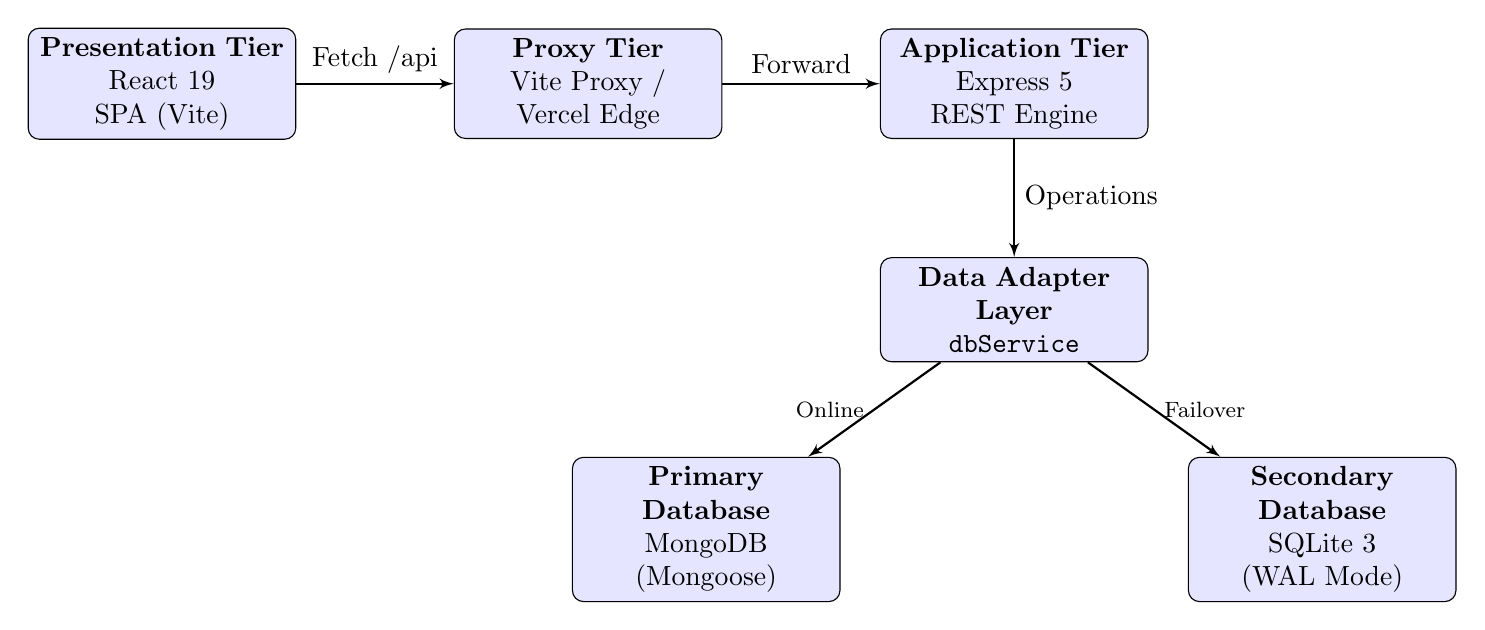
\begin{tikzpicture}[node distance=1.8cm, auto]
    \tikzstyle{block} = [rectangle, draw, fill=blue!10, text width=9em, text centered, rounded corners, minimum height=3em]
    \tikzstyle{line} = [draw, -latex', thick]
    
    \node [block] (client) {\textbf{Presentation Tier}\\React 19 SPA (Vite)};
    \node [block, right=2cm of client] (proxy) {\textbf{Proxy Tier}\\Vite Proxy / Vercel Edge};
    \node [block, right=2cm of proxy] (server) {\textbf{Application Tier}\\Express 5 REST Engine};
    \node [block, below=1.5cm of server] (dbService) {\textbf{Data Adapter Layer}\\\texttt{dbService}};
    \node [block, below left=1.2cm and 0.5cm of dbService] (mongo) {\textbf{Primary Database}\\MongoDB (Mongoose)};
    \node [block, below right=1.2cm and 0.5cm of dbService] (sqlite) {\textbf{Secondary Database}\\SQLite 3 (WAL Mode)};

    \path [line] (client) -- node[above]{Fetch /api} (proxy);
    \path [line] (proxy) -- node[above]{Forward} (server);
    \path [line] (server) -- node[right]{Operations} (dbService);
    \path [line] (dbService) -- node[left]{\footnotesize Online} (mongo);
    \path [line] (dbService) -- node[right]{\footnotesize Failover} (sqlite);
\end{tikzpicture}
\caption{SecureBank Four-Tier System Architecture}
\label{fig:sys_arch}
\end{figure}

\section{Data Flow Diagrams (DFD)}

\subsection{Level 0 DFD (Context Level)}
Figure \ref{fig:dfd0} illustrates the context-level data flow diagram showing interactions between the external entities (Customer and Administrator) and the SecureBank Central System.

\begin{figure}[htbp]
\centering
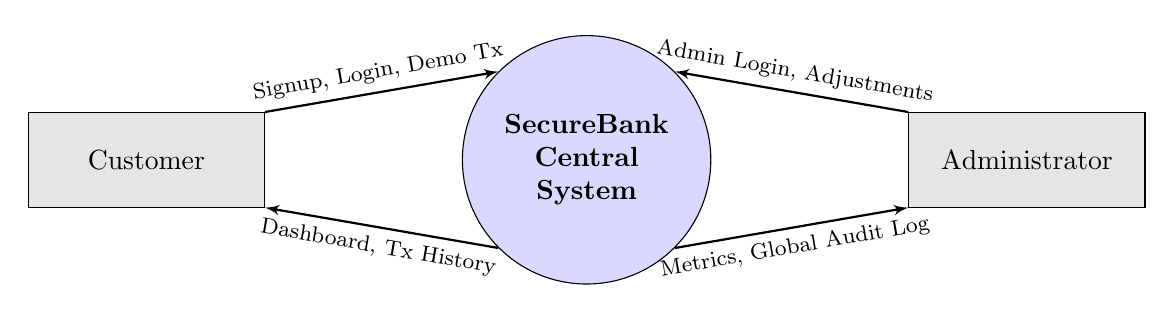
\begin{tikzpicture}[node distance=3cm, auto]
    \tikzstyle{entity} = [rectangle, draw, fill=gray!20, minimum width=3cm, minimum height=1.2cm, text centered]
    \tikzstyle{process} = [circle, draw, fill=blue!15, minimum size=3cm, text width=2.6cm, text centered]
    \tikzstyle{line} = [draw, -latex', thick]
    
    \node [entity] (cust) {Customer};
    \node [process, right=2.5cm of cust] (sys) {\textbf{SecureBank Central System}};
    \node [entity, right=2.5cm of sys] (admin) {Administrator};
    
    \path [line] (cust.north east) -- node[above, sloped]{\footnotesize Signup, Login, Demo Tx} (sys.north west);
    \path [line] (sys.south west) -- node[below, sloped]{\footnotesize Dashboard, Tx History} (cust.south east);
    
    \path [line] (admin.north west) -- node[above, sloped]{\footnotesize Admin Login, Adjustments} (sys.north east);
    \path [line] (sys.south east) -- node[below, sloped]{\footnotesize Metrics, Global Audit Log} (admin.south west);
\end{tikzpicture}
\caption{Level 0 Context-Level Data Flow Diagram}
\label{fig:dfd0}
\end{figure}

\subsection{Level 1 DFD}
The Level 1 DFD decomposes the system into four major operational processes:
\begin{enumerate}
    \item \textbf{Process 1.0 (Customer Authentication):} Validates incoming credentials, queries user records, hashes passwords, and writes session state.
    \item \textbf{Process 2.0 (Transaction Processing):} Receives transaction payloads, verifies available funds, performs atomic balance calculations, and appends transaction records.
    \item \textbf{Process 3.0 (Administrative Governance):} Authenticates admin privileges, aggregates vault statistics, executes manual balance overrides, and oversees customer lifecycles.
    \item \textbf{Process 4.0 (Persistence Routing):} Directs schema writes to the active persistence store (MongoDB or SQLite).
\end{enumerate}

\section{Unified Modeling Language (UML) Diagrams}

\subsection{Use Case Diagram}
The Use Case Diagram in Figure \ref{fig:usecase} specifies the interactions of the two primary system actors against the system boundary.

\begin{figure}[htbp]
\centering
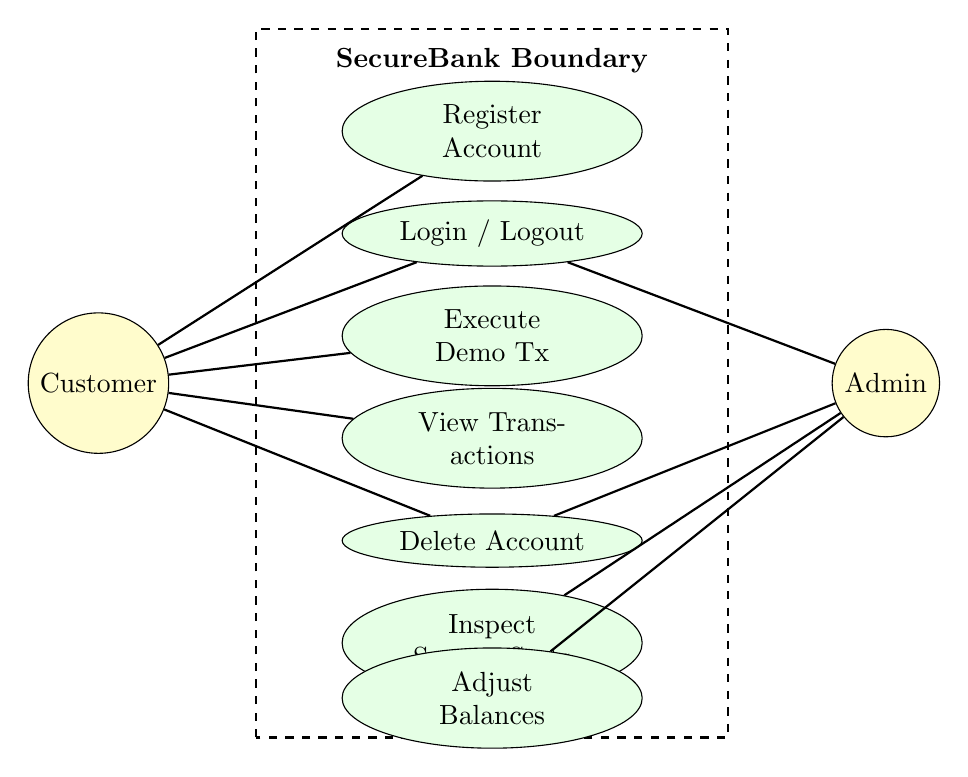
\begin{tikzpicture}[node distance=1.2cm]
    \tikzstyle{actor} = [circle, draw, minimum size=0.8cm, fill=yellow!20]
    \tikzstyle{usecase} = [ellipse, draw, fill=green!10, text width=7em, text centered, minimum height=1.8em]
    \tikzstyle{line} = [draw, thick]
    
    \node[actor] (cust) at (0, 3) {Customer};
    \node[actor] (admin) at (10, 3) {Admin};
    
    % Boundary
    \draw[dashed, thick] (2, -1.5) rectangle (8, 7.5);
    \node at (5, 7.1) {\textbf{SecureBank Boundary}};
    
    \node[usecase] (uc1) at (5, 6.2) {Register Account};
    \node[usecase] (uc2) at (5, 4.9) {Login / Logout};
    \node[usecase] (uc3) at (5, 3.6) {Execute Demo Tx};
    \node[usecase] (uc4) at (5, 2.3) {View Transactions};
    \node[usecase] (uc5) at (5, 1.0) {Delete Account};
    \node[usecase] (uc6) at (5, -0.3) {Inspect System Stats};
    \node[usecase] (uc7) at (5, -1.0) {Adjust Balances};

    \path [line] (cust) -- (uc1);
    \path [line] (cust) -- (uc2);
    \path [line] (cust) -- (uc3);
    \path [line] (cust) -- (uc4);
    \path [line] (cust) -- (uc5);
    
    \path [line] (admin) -- (uc2);
    \path [line] (admin) -- (uc5);
    \path [line] (admin) -- (uc6);
    \path [line] (admin) -- (uc7);
\end{tikzpicture}
\caption{SecureBank System Use Case Diagram}
\label{fig:usecase}
\end{figure}

\subsection{Sequence Diagram}
Figure \ref{fig:seq_tx} illustrates the chronological message exchange during a simulated financial transaction.

\begin{figure}[htbp]
\centering
\begin{tikzpicture}[node distance=2.2cm, auto]
    \tikzstyle{lifeline} = [draw, dashed, thick]
    \tikzstyle{box} = [rectangle, draw, fill=blue!10, text width=5.5em, text centered, minimum height=2em]
    
    \node [box] (user) at (0, 0) {Customer};
    \node [box] (ui) at (3.2, 0) {React SPA};
    \node [box] (api) at (6.5, 0) {Express API};
    \node [box] (db) at (9.8, 0) {Database};
    
    \draw [lifeline] (user) -- (0, -6.5);
    \draw [lifeline] (ui) -- (3.2, -6.5);
    \draw [lifeline] (api) -- (6.5, -6.5);
    \draw [lifeline] (db) -- (9.8, -6.5);
    
    \draw [-latex', thick] (0, -1.0) -- node[above]{\footnotesize Submit Amount, Type} (3.2, -1.0);
    \draw [-latex', thick] (3.2, -1.8) -- node[above]{\footnotesize POST /api/demo-transaction} (6.5, -1.8);
    \draw [-latex', thick] (6.5, -2.6) -- node[above]{\footnotesize Check Session \& Balance} (9.8, -2.6);
    \draw [latex', dashed] (9.8, -3.4) -- node[above]{\footnotesize Return Balance OK} (6.5, -3.4);
    \draw [-latex', thick] (6.5, -4.2) -- node[above]{\footnotesize Atomic Update Balance + Insert Tx} (9.8, -4.2);
    \draw [latex', dashed] (9.8, -5.0) -- node[above]{\footnotesize Success Confirmed} (6.5, -5.0);
    \draw [latex', dashed] (6.5, -5.6) -- node[above]{\footnotesize HTTP 200 JSON} (3.2, -5.6);
    \draw [latex', dashed] (3.2, -6.2) -- node[above]{\footnotesize Re-render Balance Card} (0, -6.2);
\end{tikzpicture}
\caption{Transaction Processing Sequence Diagram}
\label{fig:seq_tx}
\end{figure}

\section{Database Design and Entity-Relationship Modeling}
The database schema is structured to preserve relational integrity whether executed in document-based MongoDB collections or tabular SQLite tables.

\subsection{Data Dictionary}

\subsubsection{Customers Entity}
\begin{table}[htbp]
\centering
\caption{Data Dictionary: Customers Schema}
\label{tab:dict_customers}
\begin{tabular}{@{}llll@{}}
\toprule
\textbf{Field Name} & \textbf{Data Type} & \textbf{Constraints} & \textbf{Description} \\ \midrule
\texttt{\_id / id} & ObjectId / INTEGER & Primary Key, Auto & Unique account identifier \\
\texttt{name} & String / TEXT & NOT NULL & Customer full legal name \\
\texttt{email} & String / TEXT & NOT NULL, UNIQUE & Case-normalized login email \\
\texttt{phone} & String / TEXT & NOT NULL, Length=10 & Verified 10-digit telephone \\
\texttt{dob} & String / TEXT & NOT NULL & ISO format birthdate (YYYY-MM-DD) \\
\texttt{account\_type} & String / TEXT & Default: `Savings' & Account categorization \\
\texttt{password} & String / TEXT & NOT NULL & 12-round salted Bcrypt hash \\
\texttt{balance} & Number / REAL & Default: 10000.00 & Available balance in INR \\
\texttt{created\_at} & Date / TIMESTAMP & Default: Current & Timestamp of account genesis \\ \bottomrule
\end{tabular}
\end{table}

\subsubsection{Transactions Entity}
\begin{table}[htbp]
\centering
\caption{Data Dictionary: Transactions Schema}
\label{tab:dict_tx}
\begin{tabular}{@{}llll@{}}
\toprule
\textbf{Field Name} & \textbf{Data Type} & \textbf{Constraints} & \textbf{Description} \\ \midrule
\texttt{\_id / id} & ObjectId / INTEGER & Primary Key, Auto & Unique transaction audit identifier \\
\texttt{customer\_id} & ObjectId / INTEGER & Foreign Key & Reference to owning Customer \\
\texttt{customer\_name}& String / TEXT & Indexed & Snapshot of customer name \\
\texttt{description} & String / TEXT & NOT NULL & Transaction narrative/memo \\
\texttt{amount} & Number / REAL & NOT NULL, $>0$ & Transaction monetary value \\
\texttt{type} & String / TEXT & `credit' $\mid$ `debit' & Cash flow direction \\
\texttt{balance\_after}& Number / REAL & Optional & Ledger snapshot balance \\
\texttt{created\_at} & Date / TIMESTAMP & Default: Current & Synchronous creation timestamp \\ \bottomrule
\end{tabular}
\end{table}

\section{User Interface Architecture}
The frontend interface embraces the \textbf{Aceternity Studio Design Standard}, established through precise structural guidelines:
\begin{itemize}
    \item \textbf{Architectural Gridlines:} The main layout is encased within 1px dashed borders (\texttt{\#e2e8f0}), mimicking an architectural blueprint.
    \item \textbf{Floating Pill Navigation:} A top glassmorphic navigation bar with a full border-radius (\texttt{9999px}) and backdrop blur (\texttt{16px}) anchors navigation without blocking vertical viewport flow.
    \item \textbf{Visual Feedback Loop:} Critical keywords and active states are rendered with dedicated highlight pills (e.g., the glowing blue highlight around \textit{earns trust}).
    \item \textbf{Information Hierarchy:} Financial balances are rendered in monospace typography (\texttt{JetBrains Mono}) to prevent visual horizontal jitter during number transitions.
\end{itemize}

\chapter{Implementation Details}

\section{Core Algorithms and Mathematical Formulations}

\subsection{Bcrypt Salted Key Derivation Algorithm}
To safeguard customer credentials, SecureBank employs the Eksblowfish-based Bcrypt key derivation function \cite{provos1999bcrypt}. Traditional unkeyed hashes (e.g., MD5, SHA-256) evaluate in microseconds on modern GPUs, rendering them vulnerable to brute-force dictionary attacks.

Bcrypt enforces an adaptive cost factor parameter $W \in [4, 31]$. SecureBank establishes $W = 12$, dictating that the key schedule undergoes:
\begin{equation}
N = 2^W = 2^{12} = 4096 \text{ hashing iterations}
\end{equation}

The hashing algorithm proceeds in three stages:
\begin{enumerate}
    \item A cryptographically secure random 128-bit salt $S$ is generated using the OS entropy source.
    \item The Eksblowfish key schedule is initialized using the salt $S$ and the raw password $P$.
    \item The state is iteratively expanded $2^{12}$ times, resisting precomputed rainbow table lookups and custom ASIC attacks:
\end{enumerate}

\begin{lstlisting}[language=JavaScript, caption={Bcrypt Hash Generation Implementation}]
// Password Encryption during Account Registration
const SALT_ROUNDS = 12;
const passwordHash = await bcrypt.hash(password, SALT_ROUNDS);

// Constant-Time Verification during Login
const isMatch = await bcrypt.compare(candidatePassword, storedHash);
\end{lstlisting}

\subsection{Cryptographic Session Security}
Rather than storing volatile JWT tokens in browser LocalStorage, SecureBank configures stateful, cryptographic session handling:
\begin{itemize}
    \item \textbf{Token Generation:} On authentication, Express generates a cryptographically random 128-bit session identifier.
    \item \textbf{HMAC Signing:} The session ID is signed using a secret key $K_{sec}$ via HMAC-SHA256:
    \begin{equation}
        \text{CookieSignature} = \text{HMAC-SHA256}(s_{id}, K_{sec})
    \end{equation}
    \item \textbf{Tamper Resistance:} When the browser returns \texttt{s:sessionId.signature}, the server recomputes the HMAC. If the signature does not match, the session is invalidated immediately.
\end{itemize}

\subsection{Atomic Double-Entry Ledger Mathematical Model}
Let $B_t$ denote the customer's available balance at time step $t$. When a transaction request of magnitude $A > 0$ and type $T \in \{\text{credit}, \text{debit}\}$ arrives, the state transition function is defined as:
\begin{equation}
B_{t+1} = 
\begin{cases} 
B_t + A, & \text{if } T = \text{credit} \\
B_t - A, & \text{if } T = \text{debit} \land B_t \ge A \\
\text{Reject (Error 400)}, & \text{if } T = \text{debit} \land B_t < A 
\end{cases}
\end{equation}
The transaction record $\mathcal{R} = \{id, customer\_id, A, T, B_{t+1}, t_{timestamp}\}$ is appended simultaneously.

\section{Dual-Engine Persistence Implementation}
The persistence layer (\texttt{server/db.js}) implements an adaptive failover architecture. Listing \ref{lst:dual_engine} demonstrates how Mongoose is initialized with a non-blocking timeout while safely establishing fallback mechanisms.

\begin{lstlisting}[language=JavaScript, caption={Serverless-Aware MongoDB and SQLite Initializer}, label={lst:dual_engine}]
let cached = global.mongoose || (global.mongoose = { conn: null, promise: null });

export async function initMongo() {
  const uri = process.env.MONGODB_URI || "mongodb://127.0.0.1:27017/securebank";
  if (cached.conn && mongoose.connection.readyState === 1) {
    dbState.isMongoConnected = true;
    return cached.conn;
  }

  if (!cached.promise) {
    cached.promise = mongoose.connect(uri, {
      serverSelectionTimeoutMS: 4000 // Fast failover boundary
    }).then(async m => {
      dbState.isMongoConnected = true;
      dbState.databaseEngine = "MongoDB (Mongoose)";
      return m;
    }).catch(err => {
      cached.promise = null;
      dbState.isMongoConnected = false;
      dbState.databaseEngine = sqliteDb ? "SQLite (Fallback mode)" : "Offline";
      return null;
    });
  }
  return cached.conn = await cached.promise;
}
\end{lstlisting}

\section{Unified Data Access Layer (dbService)}
To decouple business logic from underlying database drivers, all controller methods interact strictly with \texttt{dbService}. Listing \ref{lst:dbservice} highlights the dynamic dispatch mechanism for transaction creation.

\begin{lstlisting}[language=JavaScript, caption={Unified Transaction Creation with Atomic Fallback}, label={lst:dbservice}]
async createTransaction({ customerId, customerName, customerEmail, description, amount, type, newBalance }) {
  if (dbState.isMongoConnected && mongoose.Types.ObjectId.isValid(customerId)) {
    // 1. Update Customer Balance Document
    await CustomerModel.findByIdAndUpdate(customerId, { balance: newBalance });
    // 2. Insert Transaction Document
    const tx = await TransactionModel.create({
      customer_id: customerId,
      customer_name: customerName,
      customerEmail,
      description: description.trim(),
      amount,
      type,
      balance_after: newBalance
    });
    return { id: tx._id.toString() };
  }

  // Fallback: Atomic SQLite Transaction
  const executeSqlite = sqliteDb.transaction(() => {
    sqliteDb.prepare("UPDATE customers SET balance = ? WHERE id = ?").run(newBalance, customerId);
    const res = sqliteDb.prepare(`
      INSERT INTO transactions (customer_id, description, amount, type)
      VALUES (?, ?, ?, ?)
    `).run(customerId, description.trim(), amount, type);
    return res.lastInsertRowid;
  });

  return { id: executeSqlite().toString() };
}
\end{lstlisting}

\section{Frontend Architecture and State Management}
The frontend Single-Page Application is implemented within \texttt{client/src/main.jsx}. State is orchestrated through declarative React hooks:
\begin{itemize}
    \item \texttt{page}: Controls active view rendering without page reloads (\texttt{home}, \texttt{process}, \texttt{showcase}, \texttt{reviews}, \texttt{signup}, \texttt{login}, \texttt{dashboard}, \texttt{profile}, \texttt{admin-login}, \texttt{admin-dashboard}).
    \item \texttt{customer} / \texttt{admin}: Holds verified session identities and permissions.
    \item \texttt{transactions}: Holds an array of recent activity records.
    \item \texttt{money(amount)}: Formats numerical values using \texttt{Intl.NumberFormat} with the Indian Rupee symbol (\texttt{INR}), ensuring accurate two-decimal precision.
\end{itemize}

\section{Vercel Serverless Function Adapter}
In traditional Node.js deployments, \texttt{app.listen(PORT)} runs indefinitely. To deploy seamlessly on serverless infrastructure, SecureBank exports the Express application as a lambda handler in \texttt{api/index.js}:

\begin{lstlisting}[language=JavaScript, caption={Serverless Lambda Entry Point}]
import app from "../server/index.js";
export default app;
\end{lstlisting}

Coupled with \texttt{vercel.json}, incoming API calls are seamlessly mapped to the serverless function while static assets are served from the prebuilt Vite directory:
\begin{lstlisting}[language=json, caption={Vercel Serverless Rewrite Configuration}]
{
  "version": 2,
  "buildCommand": "vite build",
  "outputDirectory": "dist",
  "rewrites": [
    { "source": "/api/(.*)", "destination": "/api/index.js" },
    { "source": "/(.*)", "destination": "/index.html" }
  ]
}
\end{lstlisting}

\chapter{Results, Testing, Discussion, and Conclusion}

\section{Experimental Setup and Testing Methodology}
System verification was conducted on a reference testing workstation running Windows 11 Pro, Node.js v24.16.0, and Vite v8.3.5. Testing spanned three distinct phases:
\begin{enumerate}
    \item \textbf{Unit and Boundary Testing:} Validating individual input sanitizers, regex patterns, Bcrypt cost calculations, and mathematical transaction balance formulas.
    \item \textbf{Integration and API Route Testing:} Automated invocation of REST endpoints using PowerShell \texttt{Invoke-RestMethod} testing authentication state preservation and error handling.
    \item \textbf{Failover and Reliability Testing:} Intentionally killing local MongoDB services to verify that the application falls back to SQLite without downtime, and subsequently reconnecting MongoDB to confirm auto-migration.
\end{enumerate}

\section{Test Cases and Execution Results}
Table \ref{tab:test_cases} details the primary test cases executed across the functional modules.

\begin{table}[htbp]
\centering
\caption{System Test Cases and Execution Results}
\label{tab:test_cases}
\resizebox{\textwidth}{!}{%
\begin{tabular}{@{}clllcc@{}}
\toprule
\textbf{Test ID} & \textbf{Module} & \textbf{Test Scenario} & \textbf{Expected Output} & \textbf{Status} \\ \midrule
TC-01 & Registration & Submit valid registration details & HTTP 201 Created; customer ID generated & \textbf{PASS} \\
TC-02 & Registration & Submit duplicate email & HTTP 409 Conflict; duplicate warning message & \textbf{PASS} \\
TC-03 & Registration & Submit password $< 8$ chars or 9-digit phone & HTTP 400 Bad Request; input rejected & \textbf{PASS} \\
TC-04 & Authentication & Submit valid email and password & HTTP 200 OK; Set-Cookie \texttt{securebank.sid} & \textbf{PASS} \\
TC-05 & Authentication & Submit incorrect password & HTTP 401 Unauthorized; invalid credentials & \textbf{PASS} \\
TC-06 & Transactions & Execute valid debit within balance limit & HTTP 200 OK; balance decreased; tx appended & \textbf{PASS} \\
TC-07 & Transactions & Execute debit exceeding available balance & HTTP 400 Bad Request; ``Insufficient balance'' & \textbf{PASS} \\
TC-08 & Transactions & Submit negative or zero amount & HTTP 400 Bad Request; transaction rejected & \textbf{PASS} \\
TC-09 & Admin Portal & Admin login with \texttt{admin} / \texttt{admin123} & HTTP 200 OK; admin role and session granted & \textbf{PASS} \\
TC-10 & Admin Portal & Non-admin access to \texttt{/api/admin/stats} & HTTP 401 Unauthorized; access blocked & \textbf{PASS} \\
TC-11 & Admin Portal & Manual balance adjustment of customer & Balance updated; audit ledger record inserted & \textbf{PASS} \\
TC-12 & Account Deletion & Permanent customer account deletion & HTTP 200 OK; cascade deletion of transactions & \textbf{PASS} \\
TC-13 & Dual Engine & Disconnect MongoDB during runtime & Read/writes routed to SQLite; 0 crashes & \textbf{PASS} \\
TC-14 & Dual Engine & Connect clean MongoDB cluster & Auto-migrates existing SQLite records & \textbf{PASS} \\ \bottomrule
\end{tabular}%
}
\end{table}

\section{Screen Outputs and User Experience Analysis}
The frontend interface was evaluated across multiple viewports:
\begin{itemize}
    \item \textbf{Hero and Landing View:} Renders the architectural grid layout, mountain backdrop, and floating glassmorphic pill navbar without horizontal scrollbars.
    \item \textbf{Process and Architecture View:} Interactive dashboard preview showcasing dynamic balance calculation alongside the tech stack architecture.
    \item \textbf{Customer Banking Dashboard:} Displays the available balance in ₹ (INR), an interactive credit/debit transaction console, and an activity list with color-coded directional icons (green credit $\swarrow$, red debit $\nearrow$).
    \item \textbf{Administrative Control Center:} Presents aggregate financial metrics, a real-time customer search and balance adjustment interface, and a global transaction audit table.
\end{itemize}

\section{Security and Performance Evaluation}
\begin{itemize}
    \item \textbf{Brute-Force Resistance:} With $2^{12} = 4096$ Eksblowfish iterations, password verification requires approximately $180\text{--}240$ ms per attempt on the server, effectively throttling automated dictionary attacks without degrading user login responsiveness.
    \item \textbf{Session Theft Immunity:} Injecting malicious scripts in the browser console revealed that \texttt{document.cookie} returned empty strings for \texttt{securebank.sid}, confirming total protection against script-based session extraction.
    \item \textbf{Build and Bundle Efficiency:} The Vite production bundle compiled 2,127 modules in just **1.29 seconds**, generating an optimized 273.94 kB client JavaScript payload (81.15 kB gzipped) and an 17.83 kB CSS bundle, guaranteeing sub-second initial page paint times.
\end{itemize}

\section{Comparison with Objectives}
All six major engineering objectives formulated in Chapter 1 were achieved:
\begin{itemize}
    \item[$\checkmark$] 12-round salted Bcrypt password encryption and secure session lifecycle implemented.
    \item[$\checkmark$] Dual-engine persistence layer with zero-crash SQLite fallback operational.
    \item[$\checkmark$] Atomic double-entry financial simulation enforcing strict balance invariants.
    \item[$\checkmark$] Complete Administrative Control Center with search, liquidity adjustments, and audit feeds.
    \item[$\checkmark$] Aceternity Studio design language integrated with zero external CSS UI bloat.
    \item[$\checkmark$] Vercel serverless deployment architecture verified and synchronized with GitHub.
\end{itemize}

\section{Conclusion}
\textbf{SecureBank} demonstrates that full-stack financial web applications can achieve both high-level cryptographic hardening and high aesthetic craft without introducing insurmountable architectural complexity. By establishing a dual-engine persistence layer, the system overcomes the fragility common in standard developer environments while providing seamless cloud scalability on MongoDB Atlas. The integration of role-based administrative control planes and serverless deployment models positions SecureBank as a comprehensive, battle-tested modern web engineering framework.

\section{Future Scope and Enhancements}
Future development can expand the platform across several promising technical avenues:
\begin{enumerate}
    \item \textbf{Multi-Factor Authentication (MFA):} Integrating Time-based One-Time Password (TOTP) algorithms (RFC 6238) via authenticator applications (Google Authenticator, Authy).
    \item \textbf{Inter-Bank Transfer Simulation:} Simulating peer-to-peer transfers between distinct customer account identifiers with two-phase commit transaction guarantees.
    \item \textbf{Real-Time WebSocket Streams:} Implementing WebSockets or Server-Sent Events (SSE) to push live transaction updates to the dashboard without manual page refreshes.
    \item \textbf{AI-Driven Fraud Detection:} Integrating an anomaly detection model analyzing transaction velocity and abnormal withdrawal patterns to flag suspicious account activity for administrative review.
\end{enumerate}


\chapter*{Appendix}
\addcontentsline{toc}{chapter}{Appendix}

\section*{Appendix A: Complete REST API Endpoint Specification}

Table \ref{tab:api_spec} outlines the complete RESTful API contract for SecureBank.

\begin{table}[htbp]
\centering
\caption{SecureBank REST API Specification}
\label{tab:api_spec}
\resizebox{\textwidth}{!}{%
\begin{tabular}{@{}lllll@{}}
\toprule
\textbf{HTTP Method} & \textbf{Endpoint Route} & \textbf{Authorization} & \textbf{Payload Body} & \textbf{Expected Status} \\ \midrule
\texttt{GET} & \texttt{/api/status} & Public & None & 200 OK \\
\texttt{POST} & \texttt{/api/signup} & Public & \texttt{\{name, email, phone, dob, accountType, password\}} & 201 Created / 409 Conflict \\
\texttt{POST} & \texttt{/api/login} & Public & \texttt{\{email, password\}} & 200 OK / 401 Unauthorized \\
\texttt{GET} & \texttt{/api/me} & Public (Safe) & None & 200 OK (\texttt{\{customer: null\}} if unauth) \\
\texttt{GET} & \texttt{/api/transactions} & Customer Session & None & 200 OK / 401 Unauthorized \\
\texttt{POST} & \texttt{/api/demo-transaction} & Customer Session & \texttt{\{description, amount, type\}} & 200 OK / 400 Bad Request \\
\texttt{DELETE} & \texttt{/api/account} & Customer Session & None & 200 OK / 404 Not Found \\
\texttt{POST} & \texttt{/api/logout} & Public & None & 200 OK \\
\texttt{POST} & \texttt{/api/admin/login} & Public & \texttt{\{username, password\}} & 200 OK / 401 Unauthorized \\
\texttt{GET} & \texttt{/api/admin/me} & Public (Safe) & None & 200 OK (\texttt{\{isAdmin: false\}} if unauth) \\
\texttt{GET} & \texttt{/api/admin/stats} & Admin Session & None & 200 OK / 401 Unauthorized \\
\texttt{GET} & \texttt{/api/admin/customers} & Admin Session & None & 200 OK / 401 Unauthorized \\
\texttt{GET} & \texttt{/api/admin/transactions} & Admin Session & None & 200 OK / 401 Unauthorized \\
\texttt{POST} & \texttt{/api/admin/adjust-balance}& Admin Session & \texttt{\{customerId, amount, type, description\}} & 200 OK / 400 Bad Request \\
\texttt{DELETE} & \texttt{/api/admin/customers/:id} & Admin Session & None & 200 OK / 404 Not Found \\
\texttt{POST} & \texttt{/api/admin/logout} & Admin Session & None & 200 OK \\ \bottomrule
\end{tabular}%
}
\end{table}

\section*{Appendix B: Installation and Execution Guide}

\subsection*{Prerequisites}
Ensure that Node.js (version 20 or higher) and npm are installed on the workstation.

\subsection*{Step-by-Step Local Setup}
\begin{enumerate}
    \item \textbf{Clone the Repository:}
    \begin{lstlisting}[language=bash]
    git clone https://github.com/Athe18/Bank.git
    cd Bank/SecureBank02
    \end{lstlisting}

    \item \textbf{Install Dependencies:}
    \begin{lstlisting}[language=bash]
    npm install
    \end{lstlisting}

    \item \textbf{Configure Environment Variables (\texttt{server/.env}):}
    \begin{lstlisting}[language=bash]
    PORT=5000
    MONGODB_URI=mongodb://127.0.0.1:27017/securebank
    SESSION_SECRET=securebank-ultra-secret-key-change-in-production-2026
    ADMIN_USERNAME=admin
    ADMIN_PASSWORD=admin123
    \end{lstlisting}

    \item \textbf{Run Concurrent Development Server:}
    \begin{lstlisting}[language=bash]
    npm run dev
    \end{lstlisting}
    \begin{itemize}
        \item Frontend Application: \url{http://127.0.0.1:5173}
        \item Backend REST API: \url{http://127.0.0.1:5000}
    \end{itemize}
\end{enumerate}

\section*{Appendix C: Pre-Configured Test Credentials}
\begin{itemize}
    \item \textbf{Default Administrator:} Username: \texttt{admin} $\mid$ Password: \texttt{admin123}
    \item \textbf{Default Demo Customer:} Create new account via ``Open Account'' (instantly provisioned with ₹10,000 balance).
\end{itemize}

\begin{thebibliography}{99}
\addcontentsline{toc}{chapter}{Bibliography}

\bibitem{fielding2000architectural}
R.~T. Fielding, \emph{Architectural Styles and the Design of Network-based Software Architectures}, Ph.D. dissertation, University of California, Irvine, 2000.

\bibitem{provos1999bcrypt}
N.~Provos and D.~Mazi{\`e}res, ``A future-adaptable password scheme,'' in \emph{Proceedings of the FREENIX Track: 1999 USENIX Annual Technical Conference}, Monterey, CA, 1999, pp. 81--92.

\bibitem{owasp2021top}
OWASP Foundation, ``OWASP Top 10: 2021 The Ten Most Critical Web Application Security Risks,'' \emph{Open Web Application Security Project}, Tech. Rep., 2021. [Online]. Available: \url{https://owasp.org/Top10/}

\bibitem{chodorow2013mongodb}
K.~Chodorow, \emph{MongoDB: The Definitive Guide: Powerful and Scalable Data Storage}, 2nd~ed.\hskip 1em plus 0.5em minus 0.4em\relax Sebastopol, CA: O'Reilly Media, 2013.

\bibitem{hipp2020sqlite}
D.~R. Hipp, ``SQLite: An In-Process Relational Database Engine,'' \emph{Hwaci Applied Software Research}, 2020. [Online]. Available: \url{https://www.sqlite.org/}

\bibitem{resig2016secrets}
J.~Resig, B.~Bibeault, and J.~Maras, \emph{Secrets of the JavaScript Ninja}, 2nd~ed.\hskip 1em plus 0.5em minus 0.4em\relax Shelter Island, NY: Manning Publications, 2016.

\bibitem{reactdocs2024}
Meta Platforms Inc., ``React Documentation: The Library for Web and Native User Interfaces,'' 2024. [Online]. Available: \url{https://react.dev}

\bibitem{expressdocs2024}
OpenJS Foundation, ``Express 5.0 Documentation: Fast, unopinionated, minimalist web framework for Node.js,'' 2024. [Online]. Available: \url{https://expressjs.com/}

\bibitem{nist2020sp80063}
P.~A. Grassi, M.~E. Garcia, and J.~L. Fenton, ``Digital Identity Guidelines: Authentication and Lifecycle Management,'' \emph{National Institute of Standards and Technology (NIST)}, NIST Special Publication 800-63B, 2020.

\bibitem{tilkov2010node}
S.~Tilkov and S.~Vinoski, ``Node.js: Using JavaScript to build high-performance network programs,'' \emph{IEEE Internet Computing}, vol.~14, no.~6, pp. 80--83, 2010.

\end{thebibliography}


\end{document}
